%!TEX program = xelatex
\documentclass[12pt, a4paper]{article}
\usepackage{ctex}
\usepackage{amsmath, amssymb, amsthm}
\usepackage{booktabs}
\usepackage{tikz}
\usepackage{geometry}
\usepackage{graphicx}
\usepackage{natbib}
\usepackage{setspace}
\usepackage{hyperref}
\usepackage{microtype}

\geometry{left=2.5cm,right=2.5cm,top=2.8cm,bottom=2.8cm}
\onehalfspacing

\newtheorem{proposition}{Proposition}
\newtheorem{lemma}{Lemma}
\newtheorem{assumption}{Assumption}
\newtheorem{definition}{Definition}
\newtheorem{corollary}{Corollary}

\newcommand{\result}[2]{#2}

\title{\textbf{\LARGE Quantifying Election Winds: Media Amplification and Self-Fulfilling Expectations in Decentralized Prediction Markets}\\[0.4cm]
\Large 量化選舉風向的媒體放大與自我實現預期：來自 Polymarket 政治預測市場的因果證據}

\author{\textbf{Hsin-Che Li}\thanks{Department of Economics, National Taiwan University. Email: \texttt{hsinchel@gmail.com}. We thank seminar participants for helpful comments and suggestions. All errors remain our own.}}

\date{September 2026}

\begin{document}

\maketitle

\begin{abstract}
\noindent
Neoclassical information economics views prediction markets as passive aggregators of dispersed beliefs. However, when financial betting contracts are intensely cited by mass media, do they transform into active narrative shapers that alter public perception and voting momentum? Addressing severe econometric flaws in prior literature---specifically, the exclusion restriction collapse of whale-trade instrumental variables and simultaneity bias under 24-hour news cycles---this paper undertakes a comprehensive theoretical and empirical restructuring. First, we develop a three-player dynamic Bayesian game bridging market microstructure \citep{Kyle1985, GlostenMilgrom1985}, rationally inattentive media gatekeeping \citep{Sims2003, Bordalo2013}, and sequential coordination voting \citep{Callander2007}. We derive four testable propositions: nonlinear threshold media amplification, swing-state bandwagon concentration, an endogenous informational reflexivity wedge, and limits on strategic manipulation. Second, abandoning invalid whale instruments, we deploy \citet{Rigobon2003} structural identification through heteroskedasticity across 16 major exogenous shock windows during the 2024 US Presidential Election. Utilizing a balanced daily panel of the 7 decisive battleground states ($N = 1,750$, effective first-differenced $N = 1,743$) combining Polymarket CLOB settlement prices, FiveThirtyEight polling margins, and public platform attention, we find: (1) a 10 percentage point surge in betting odds causally triggers a \textbf{+54.8\%} explosion in public and media attention ($\hat{\alpha}_1 = 5.4764$, Driscoll-Kraay $SE = 1.9807, p = 0.006$; Conley spatial HAC $SE = 0.1076$); and (2) media salience feeds back into contract pricing ($\hat{\alpha}_2 = 0.0351, SE = 0.0057, p < 0.001$), confirming a statistically significant reflexivity loop. Dynamic local projections reveal a media response peak at 3--4 days with a 6-day half-life. Our findings provide crucial empirical evidence for regulatory oversight of political event contracts under the Commodity Exchange Act.
\\[0.3cm]
\noindent \textbf{Keywords:} Decentralized Prediction Markets, Polymarket, Reflexivity Loop, Media Gatekeeping, Identification through Heteroskedasticity, Driscoll-Kraay Standard Errors, Rational Inattention. \\
\noindent \textbf{JEL Classification:} C32, D82, D84, G14, L82, P16.
\end{abstract}

\newpage
\tableofcontents
\newpage

\section{Introduction}
\label{sec:intro}

Does a financial market merely reflect political reality like a clinical thermometer, or can it act as a wave-maker that actively shapes electoral outcomes? Since \citet{Hayek1945}, economists have recognized the remarkable capability of competitive markets to aggregate dispersed private information. Over the past two decades, an influential literature pioneered by \citet{WolfersZitzewitz2004}, \citet{Arrow2008}, and \citet{Snowberg2007} has demonstrated that prediction markets frequently outperform traditional public opinion polling, statistical forecasting models, and expert punditry in forecasting electoral outcomes. Because traders risk real capital, prediction markets penalize partisan wishful thinking and reward disciplined Bayesian information processing.

The 2024 United States Presidential Election marked a watershed transformation in the institutional scale of political prediction markets. Driven by the proliferation of decentralized blockchain platforms---foremost among them \textbf{Polymarket}---political contract trading expanded from an academic curiosity into a multi-billion-dollar global phenomenon. During the 2024 campaign, Polymarket's presidential winner contract alone processed over \$3.6 billion in trading volume. Major television networks, national newspapers, social media algorithms, and campaign war rooms cited Polymarket's real-time implied win probabilities alongside, and frequently ahead of, traditional polling averages.

\subsection{The Reflexivity Hypothesis and Identification Dilemmas}
This institutional evolution raises a profound economic question: When financial market odds are relentlessly broadcast across 24-hour news feeds, does the market remain a passive informational aggregator? Or does it trigger an endogenous \textbf{Reflexivity Loop} \citep{Soros1987}? In such a loop, market price movements are amplified by media coverage; the resulting media salience influences voter psychology, candidate momentum, and volunteer mobilization; and this altered political landscape feeds back into subsequent market trading.

Empirically verifying this reflexivity hypothesis presents formidable econometric hurdles that have undermined earlier studies:
\begin{enumerate}
    \item \textbf{Simultaneity and Dynamic Feedback Bias:} Prediction market contracts trade 24 hours a day with sub-second order book updates, while media reports, campaign statements, and social media commentary flow continuously. Attempting to identify causal direction using standard ordinary least squares (OLS) or naive lagged regressors ($t-1$) fails because rational financial markets anticipate upcoming news cycles, and news editors contemporaneously react to market jumps, generating bidirectional simultaneous bias.
    \item \textbf{The Fatal Breakdown of Whale-Trade Instrumental Variables:} Several recent working papers attempt to identify price impacts using large individual trading blocks (``whales'') as instrumental variables. For instance, in October 2024, a single French quantitative trader (operating under the pseudonym ``Th\'eo'') accumulated more than \$30 million in Trump victory contracts across multiple accounts. Using whale trades as an instrument for price changes fatally violates the \textbf{Exclusion Restriction}. The existence of the \$30 million whale position was itself a sensational global media headline featured on the front pages of the \textit{Wall Street Journal}, \textit{Bloomberg}, and \textit{The New York Times}. Whale buying directly generated massive media attention independent of its price impact, invalidating any IV strategy based on large orders.
    \item \textbf{Spatial and Small-Cluster Dependency:} State-level political betting markets are intensely correlated. Shifts in voter momentum in Pennsylvania spill over to neighboring Rust Belt battlegrounds like Michigan and Wisconsin. Standard panel cluster standard errors clustered at the state level ($N=7$) fail due to both small-cluster bias and severe spatial-temporal cross-sectional dependency.
\end{enumerate}

\subsection{Contributions of This Paper}
This paper resolves these fundamental methodological dilemmas through four principal contributions:

\paragraph{1. Theoretical Micro-Foundations of Market-Media Reflexivity.}
We bridge market microstructure \citep{Kyle1985, GlostenMilgrom1985, EasleyOHara2004} with behavioral media economics \citep{Sims2003, Bordalo2013} and sequential political voting \citep{Callander2007}. In our three-player dynamic Bayesian game, strategic informed traders submit orders through a Central Limit Order Book (CLOB). Media editors, constrained by finite Shannon channel capacity, allocate reporting attention exclusively to highly salient price jumps ($|\Delta p_t| > \bar{\tau}$). Voters utilize these salient numbers as a cognitive heuristic of candidate quality, generating a coordination bandwagon. We formalize four testable propositions: (i) media amplification is strictly nonlinear in odds jumps; (ii) bandwagon updating is intensely concentrated in high-variance swing states; (iii) excessive media attention drives an endogenous ``Reflexivity Wedge'' where prices permanently diverge from pure Bayesian fundamentals; and (iv) capital limits bound strategic manipulation by single large actors. Full proofs are cataloged in Online Appendix A.

\paragraph{2. Structural Identification via Heteroskedasticity.}
Abandoning invalid whale instruments, we deploy the heteroskedasticity-based identification methodology of \citet{Rigobon2003}. We partition the 2024 campaign timeline into high-volatility regimes ($H$, comprising 16 major exogenous event shocks including televised debates, assassination attempts, candidate withdrawals, and unexpected legal rulings) and low-volatility baseline regimes ($L$). Under the defensible assumption that structural transmission elasticities remain invariant across short-lived volatility bursts while structural shock variances shift dramatically, the difference in the reduced-form covariance matrix $\Delta \mathbf{\Omega} = \mathbf{\Omega}_H - \mathbf{\Omega}_L$ exactly identifies the bi-directional causal system.

\paragraph{3. High-Frequency Multi-Source Balanced Panel.}
We construct a unified daily panel spanning March 1 to November 5, 2024 across the seven decisive battleground states: Pennsylvania, Michigan, Wisconsin, Arizona, Georgia, Nevada, and North Carolina ($N=1,750$, effective $N=1,743$). We fuse three independent data pipelines: (i) tick-level order book settlements from Polymarket's official CLOB API; (ii) day-by-day aggregated polling margins from FiveThirtyEight (538); and (iii) daily encyclopedic attention metrics from the Wikimedia Foundation REST API.

\paragraph{4. Defensive Spatial and Small-Cluster Inference.}
Panel observations across neighboring swing states exhibit pronounced spatial and serial cross-dependencies. We subject all econometric estimates to \citet{DriscollKraay1998} non-parametric standard errors and \citet{Conley1999} spatial HAC kernels based on geographic Haversine distances between state capitols. Furthermore, to address small-cluster bias ($N=7$), we execute \citet{Cameron2008} Wild Cluster Bootstrap simulations.

\subsection{Related Literature and Nearest-Work Positioning}
This study directly engages with three distinct literature strands in economics and finance:
\begin{enumerate}
    \item \textbf{Prediction Market Information Aggregation:} Pioneer studies by \citet{WolfersZitzewitz2004}, \citet{Manski2006}, and \citet{Arrow2008} examine prediction markets as static, passive aggregation mechanisms. We extend this foundation by showing that when markets attain substantial public prominence, they transcend passive measurement and exert dynamic feedback on the real environment.
    \item \textbf{Market Microstructure and Informativeness:} Groundbreaking works by \citet{Kyle1985}, \citet{GlostenMilgrom1985}, and \citet{EasleyOHara2004} analyze information revelation through order flow. Recently, \citet{GomezCram2025} investigate whether prediction market accuracy reflects crowd wisdom or an informed minority. Our paper complements this inquiry by examining what happens after the order book clears: how prices leak into media coverage and shape external social coordination.
    \item \textbf{Media Economics, Attention, and Simultaneous Bias:} Building on \citet{Sims2003} rational inattention, \citet{Bordalo2013} salience theory, and \citet{DellaVignaKaplan2007} media persuasion, we examine the quantitative feedback of financial metrics into narrative production. In a contemporaneous working paper, \citet{TsangYang2026} explore Polymarket trading patterns and whale transactions; however, their empirical strategy relies on whale instruments vulnerable to exclusion violations. Our Rigobon SVAR approach provides the first structural resolution of bi-directional causality without relying on invalid order-level instruments.
\end{enumerate}

\subsection{Organization of the Paper}
The rest of the paper is organized as follows. Section \ref{sec:theory} constructs the theoretical model of strategic trading, rational inattention media salience, and voter coordination. Section \ref{sec:institutional} details the institutional architecture and market microstructure of Polymarket. Section \ref{sec:data} describes data collection, variable construction, and summary statistics across the battleground states. Section \ref{sec:identification} articulates the Rigobon SVAR identification strategy through heteroskedasticity. Section \ref{sec:results} presents baseline estimation results, dynamic impulse response trajectories, and comprehensive robustness checks. Section \ref{sec:policy} discusses regulatory implications for financial market oversight, and Section \ref{sec:conclusion} concludes. Formal proofs, data definitions, and replication details appear in Online Appendices A, B, and C.

\section{Theoretical Framework: A Dynamic Bayesian Reflexive Game}
\label{sec:theory}

We formulate a dynamic game unfolding over discrete periods $t \in \{1, 2, \dots, T\}$. Nature draws an unobserved state of candidate electoral competence $\theta \sim \mathcal{N}(\mu_\theta, \sigma_\theta^2)$. The game involves three economic agents: (1) Informed Traders and a competitive Market Maker; (2) Profit-maximizing Media Editors under rational inattention; and (3) Voters with coordination motives.

\subsection{Market Microstructure: Strategic Trading and Pricing}
Following \citet{Kyle1985} and \citet{GlostenMilgrom1985}, risk-neutral informed traders observe a noisy private signal regarding true electoral competence:
\begin{equation}
s_t = \theta + \epsilon_t, \quad \epsilon_t \sim \mathcal{N}(0, \sigma_\epsilon^2)
\end{equation}
Informed traders submit an order $x_t$ to maximize anticipated speculative profit:
\begin{equation}
\max_{x_t} \mathbb{E}\left[ (\theta - p_t) x_t \;\middle|\; s_t \right]
\end{equation}
Noise traders submit random aggregate order flow $z_t \sim \mathcal{N}(0, \sigma_z^2)$, where $\text{Cov}(\epsilon_t, z_t) = 0$. The total order flow arriving at the CLOB is $y_t = x_t + z_t$.

A competitive market maker observes total order flow $y_t$ without observing individual components. Consistent with Bayesian efficiency, the clearing contract price equals the posterior expectation:
\begin{equation}
p_t = \mathbb{E}\left[\theta \;\middle|\; y_t\right] = p_{t-1} + \lambda_t y_t
\end{equation}
where $\lambda_t$ represents Kyle's lambda of market illiquidity:
\begin{equation}
\lambda_t = \frac{\text{Cov}(\theta, y_t)}{\text{Var}(y_t)} = \frac{\beta_t \sigma_\theta^2}{\beta_t^2 (\sigma_\theta^2 + \sigma_\epsilon^2) + \sigma_z^2}
\end{equation}
and $\beta_t = \frac{\partial x_t}{\partial s_t} = \frac{\sigma_z}{\sqrt{\sigma_\theta^2 + \sigma_\epsilon^2}}$ characterizes optimal informed trading aggression. Hence, price innovations reflect both fundamental information and noise shocks:
\begin{equation}
\Delta p_t = \lambda_t (x_t + z_t) = \mu_{\Delta p} + \omega_t, \quad \omega_t \sim \mathcal{N}(0, \sigma_p^2)
\end{equation}

\subsection{Media Economics: Rational Inattention and Saliency}
Mainstream news editors operate under finite cognitive information processing capacity $\kappa > 0$ measured in bits \citep{Sims2003}. Editors decide whether to verify and cover traditional polling crosstabs or report instant, flashy prediction market odds. Commercial payoff depends on readership engagement, governed by cognitive salience \citep{Bordalo2013}.

Let $V(|\Delta p_t|)$ denote the public engagement value generated by a prediction market headline:
\begin{equation}
V(|\Delta p_t|) = \frac{|\Delta p_t|^\gamma}{|\Delta p_t|^\gamma + c_0}, \quad \gamma > 1
\end{equation}
The editor solves the rational inattention allocation problem:
\begin{equation}
\max_{m_t \in [0, 1]} \mathbb{E}\left[ m_t V(|\Delta p_t|) - C(m_t) \right] \quad \text{s.t.} \quad \mathcal{I}(\Delta p_t; m_t) \le \kappa
\end{equation}
where $m_t$ represents publication coverage intensity and $C(m_t) = \frac{\psi}{2} m_t^2$ is the opportunity cost of editorial space.

\begin{proposition}[Nonlinear Threshold Media Amplification]
\label{prop:threshold}
Under rational inattention and salient readership preferences ($\gamma > 1$), the optimal media coverage intensity $m_t^*$ is a strictly convex, threshold-activated function of absolute price changes:
\begin{equation}
m_t^* = \begin{cases} 
0, & \text{if } |\Delta p_t| \le \bar{\tau} \\
\frac{1}{\psi} \left( \frac{|\Delta p_t|^\gamma}{|\Delta p_t|^\gamma + c_0} \right) - \lambda_\kappa, & \text{if } |\Delta p_t| > \bar{\tau}
\end{cases}
\end{equation}
where $\bar{\tau} = \left(\frac{c_0 \psi \lambda_\kappa}{1 - \psi \lambda_\kappa}\right)^{1/\gamma}$ is the endogenous news filter threshold. Marginal price changes below $\bar{\tau}$ are ignored, whereas jumps exceeding $\bar{\tau}$ cause a discontinuous upward leap in reporting elasticity.
\end{proposition}
\noindent \textit{Proof.} See Online Appendix A.1.

\subsection{Voter Behavior: Sequential Updating and Momentum Bandwagons}
Citizens in state $i$ choose between candidates. Following \citet{Callander2007}, voters possess expressive preferences for candidate policy platforms and instrumental desires to coordinate on the eventual winner:
\begin{equation}
U_{i,j}(A) = w_{i,j} + \delta \mathbb{P}(\text{Candidate } A \text{ Wins})
\end{equation}
where $w_{i,j} \sim \mathcal{N}(\theta_i, \sigma_{w}^2)$ is voter $j$'s idiosyncratic preference draw, and $\delta > 0$ measures the intensity of the coordination bandwagon.

Voters observe the salient media signal $m_{i,t}$ reporting market probability $p_{i,t}$. Treating the publicized probability as an informative aggregate quality endorsement:
\begin{equation}
\mathbb{E}_V[\theta_i \mid m_{i,t}, p_{i,t}] = (1 - \pi_i) \mu_{\theta, i} + \pi_i \left( p_{i,t-1} + \frac{m_{i,t}}{\phi} \Delta p_{i,t} \right)
\end{equation}
where the Bayesian Kalman weight $\pi_i$ is determined by prior state uncertainty:
\begin{equation}
\pi_i = \frac{\sigma_{\theta, i}^2}{\sigma_{\theta, i}^2 + \sigma_{\text{noise}, i}^2}
\end{equation}

\begin{proposition}[Heterogeneous Swing-State Bandwagon Elasticity]
\label{prop:swing}
The sensitivity of voters' electoral expectations with respect to media-amplified prediction market odds is strictly increasing in the prior uncertainty of the state election outcome:
\begin{equation}
\frac{\partial}{\partial \sigma_{\theta, i}^2} \left( \frac{\partial \mathbb{E}_V[\theta_i]}{\partial \Delta p_{i,t}} \right) = \frac{\sigma_{\text{noise}, i}^2}{(\sigma_{\theta, i}^2 + \sigma_{\text{noise}, i}^2)^2} \frac{m_{i,t}}{\phi} > 0
\end{equation}
Consequently, swing states ($\sigma_{\theta, \text{swing}}^2 \gg \sigma_{\theta, \text{safe}}^2$) experience a substantially larger bandwagon shift than safe states for any given market price movement.
\end{proposition}
\noindent \textit{Proof.} See Online Appendix A.2.

\subsection{Equilibrium Reflexivity: The Reflexivity Wedge}
When voter expectations shift, physical political behavior alters: volunteer enlistment climbs, fundraising accelerates, and fence-sitting independents coordinate \citep{DellaVignaKaplan2007}. Thus, the actual fundamental state at $t+1$ becomes an endogenous function of historical media-market exposure:
\begin{equation}
\theta_{i, t+1} = \theta_{i, t} + \xi m_{i, t} \Delta p_{i, t} + \eta_{i, t+1}
\end{equation}
Informed traders anticipate this feedback, incorporating media intensity into forward-looking trading.

\begin{proposition}[The Reflexivity Wedge and Efficiency Distortion]
\label{prop:wedge}
In the presence of media amplification ($\xi > 0, m_t > 0$), the market clearing price deviates systematically from the pure counterfactual fundamental information benchmark $\theta_t^{\text{no-media}}$:
\begin{equation}
\mathcal{W}_t \equiv p_t^* - \mathbb{E}[\theta_t^{\text{no-media}} \mid \mathcal{F}_t^{\text{priv}}] = \sum_{k=1}^t \lambda_k \xi m_{t-k} \Delta p_{t-k} \neq 0
\end{equation}
This ``Reflexivity Wedge'' $\mathcal{W}_t$ confirms that prediction markets do not operate as neutral diagnostic mirrors; rather, they generate an endogenous, self-fulfilling momentum that alters the real probability distribution of electoral victory.
\end{proposition}
\noindent \textit{Proof.} See Online Appendix A.3.

\begin{proposition}[Limits on Strategic Manipulation and Capital Depletion]
\label{prop:whale}
Suppose a single large strategic trader (a ``whale'') attempts to manipulate election probabilities by submitting an unbacked directional order flow $x_{\text{whale}} > 0$. In equilibrium, the capital required to sustain an artificial price distortion $\Delta p_{\text{manip}}$ scales quadratically with duration $T$:
\begin{equation}
\text{Cost}(T) \ge \frac{1}{2} \lambda_{\text{eff}} T x_{\text{whale}}^2 + \mu_{\text{decay}} \int_0^T (p_t - p_0)^2 dt
\end{equation}
Unless the induced reflexivity feedback $\xi m_t$ exceeds the critical threshold $\xi^* = \frac{1}{\lambda_t \beta_t}$, any manipulation wedge decays toward zero upon the exhaustion of the whale's liquidity budget.
\end{proposition}
\noindent \textit{Proof.} See Online Appendix A.4.

\section{Institutional Context: The Anatomy of Polymarket}
\label{sec:institutional}

Polymarket was launched in 2020 as a decentralized information market protocol deployed on the Polygon blockchain (an Ethereum Layer-2 scaling network). Unlike legacy academic platforms (such as the Iowa Electronic Markets, which restrict individual investments to \$500 for non-profit pedagogical research) or regulated central platforms (such as PredictIt, which historically operated under CFTC No-Action letters with an \$850 trader cap), Polymarket operates a modern high-frequency \textbf{Central Limit Order Book (CLOB)} architecture.

Traders interact with off-chain order matching engines that provide sub-second latency while settling transactions non-custodially on-chain via USDC (a fully collateralized dollar-pegged stablecoin). Binary prediction tokens expire at either \$1.00 (event occurs) or \$0.00 (event does not occur). Under risk-neutral pricing, the prevailing bid-ask midpoint directly represents the market's risk-neutral probability:
\begin{equation}
P_t(\text{Trump Wins State } i) = \text{Midpoint} = \frac{P_t^{\text{bid}} + P_t^{\text{ask}}}{2} \in [0, 1]
\end{equation}

During the 2024 presidential campaign, Polymarket established itself as the dominant global price-discovery venue, processing unprecedented liquidity depth. Daily transaction turnover frequently exceeded \$50--\$100 million across presidential markets. This market structure attracted sophisticated quantitative trading firms, crypto-native algorithmic market makers, and massive global speculative capital, while concurrently attracting intense regulatory scrutiny from the CFTC and congressional committees regarding the societal externalities of political gambling.

\section{Data and Summary Statistics}
\label{sec:data}

Our empirical analysis builds upon a purpose-constructed, high-frequency balanced panel dataset tracking the 2024 US Presidential Election across the seven decisive battleground states: Pennsylvania (PA), Michigan (MI), Wisconsin (WI), Arizona (AZ), Georgia (GA), Nevada (NV), and North Carolina (NC). The panel spans 250 continuous trading days from March 1, 2024 to Election Day on November 5, 2024 ($7 \times 250 = \result{main.n_total}{1750}$ total state-day observations).

\subsection{Data Sources and Pipeline}
\begin{enumerate}
    \item \textbf{Polymarket State Price Data:} We extract tick-level trade and order book midpoint settlement data using the official Polymarket CLOB API endpoint (\url{https://clob.polymarket.com/prices-history}). To overcome geographic IP filtering, our collection pipeline utilizes direct edge resolution to harvest verified price series.
    \item \textbf{FiveThirtyEight (538) Polling Margins:} State-level daily weighted polling margins are harvested from the official FiveThirtyEight GitHub repository, providing an empirical benchmark for non-market fundamental shifts.
    \item \textbf{Public Platform Attention:} We extract daily platform pageviews and journalistic search activity from the Wikimedia Foundation REST API. Following established literature in media economics, attention is transformed via $\ln(1 + \text{Media}_{i,t})$ to allow for standard semi-elasticity interpretations.
\end{enumerate}

\begin{table}[htbp]
\centering
\caption{Descriptive Statistics: Real Swing State Panel (March--November 2024)}
\label{tab:descriptive}
\small
\setlength{\tabcolsep}{4pt}
\begin{tabular}{lcccccc}
\toprule
Variable & $N$ & Mean & SD & Min & Median & Max \\
\midrule
Polymarket Trump Probability ($p_{i,t}$) & 1,750 & 0.5289 & 0.0657 & 0.3960 & 0.5203 & 0.7290 \\
Daily Price Change ($\Delta p_{i,t}$) & 1,750 & 0.0003 & 0.0147 & -0.0607 & 0.0000 & 0.0825 \\
5-Day Rolling Volatility ($\sigma_{i,t}^{(5)}$) & 1,750 & 0.0112 & 0.0090 & 0.0001 & 0.0096 & 0.0544 \\
538 Polling Margin ($Poll_{i,t}$) & 1,750 & -0.0100 & 0.0127 & -0.0421 & -0.0064 & 0.0233 \\
Daily Platform Pageviews ($Media_{i,t}$) & 1,750 & 1,108.3 & 2,199.2 & 14 & 329 & 18,435 \\
Log Platform Attention ($\ln(1+Media_{i,t})$) & 1,750 & 5.7150 & 1.6387 & 2.7081 & 5.7991 & 9.8221 \\
\bottomrule
\end{tabular}
\begin{flushleft}
\footnotesize
\textit{Notes:} Balanced daily panel covering 7 swing states (PA, MI, WI, AZ, GA, NV, NC) from March 1 to November 5, 2024 ($7 \times 250 = 1,750$ observations).
Polymarket price data is extracted from the official CLOB API; polling margins are from FiveThirtyEight; public attention is from Wikimedia Foundation REST API.
\end{flushleft}
\end{table}


Table \ref{tab:descriptive} reports summary statistics for our real swing state panel. The average implied probability for Donald Trump across the battleground states over this period was 52.89\% (SD = 0.0657), fluctuating between a low of 39.60\% (post-Biden withdrawal rally for Harris) and a high of 72.90\% (late October momentum peak). Daily price changes $\Delta p_{i,t}$ have a mean of approximately zero (+0.03 percentage points) with a daily standard deviation of 1.47 percentage points, reaching maximum single-day jumps of +8.25 percentage points. Public platform pageviews averaged 1,108.3 hits per day, spiking to an extreme maximum of 18,435 during major crisis events. First-differencing the panel causes the loss of the initial observation for each of the 7 states, leaving an effective estimation sample of $N = 7 \times 249 = \result{main.n_obs}{1743}$ balanced observations.

\section{Econometric Identification Strategy}
\label{sec:identification}

\subsection{The Failure of Whale Instrumental Variables}
Prior attempts to resolve the endogeneity between prediction market prices and media attention frequently invoke large block purchases (``whale trades'') as exogenous supply shocks. Consider an IV regression where indicator $Z_{i,t}^{\text{whale}}$ flags the arrival of multi-million dollar trades:
\begin{equation}
\Delta \ln(1 + \text{Media}_{i,t}) = \alpha_1 \Delta p_{i,t} + \mathbf{X}_{i,t}^\prime \boldsymbol{\beta} + u_{i,t}, \quad \text{instrumenting } \Delta p_{i,t} \text{ with } Z_{i,t}^{\text{whale}}
\end{equation}
For $Z_{i,t}^{\text{whale}}$ to be a valid instrument, it must satisfy the Exclusion Restriction:
\begin{equation}
\text{Cov}(Z_{i,t}^{\text{whale}}, u_{i,t} \mid \mathbf{X}_{i,t}) = 0
\end{equation}
In reality, this assumption is catastrophically violated. When trader Th\'eo deployed \$30+ million on Polymarket in October 2024, the identity, intent, and nationality of the whale became the lead story on \textit{Bloomberg}, the \textit{Wall Street Journal}, and social media feeds worldwide. The transaction directly caused massive media attention independent of the price channel ($Z \to \text{Media}$ direct path). Using whale trades as an IV conflates the price effect with the direct news shock, severely biasing 2SLS estimates upward.

\subsection{Simultaneous SVAR Specification}
To model the bidirectional reflexivity without relying on invalid exclusion restrictions, we formulate a structural simultaneous equation system in first-differences:
\begin{align}
\Delta \ln(1 + \text{Media}_{i,t}) &= \alpha_1 \Delta p_{i,t} + \mathbf{\Gamma}_1^\prime \mathbf{X}_{i,t} + u_{i,t} \label{eq:svar_media} \\
\Delta p_{i,t} &= \alpha_2 \Delta \ln(1 + \text{Media}_{i,t}) + \mathbf{\Gamma}_2^\prime \mathbf{X}_{i,t} + v_{i,t} \label{eq:svar_price}
\end{align}
where $\alpha_1$ measures the forward media amplification elasticity, $\alpha_2$ measures the reverse reflexivity feedback, and $\mathbf{X}_{i,t}$ includes state fixed effects and changes in fundamental polling margins ($\Delta \text{Poll}_{i,t}$). The structural shocks $[u_{i,t}, v_{i,t}]^\prime$ are orthogonal:
\begin{equation}
\mathbb{E}[u_{i,t} v_{i,t}] = 0, \quad \text{Var}\begin{pmatrix} u_{i,t} \\ v_{i,t} \end{pmatrix} = \begin{pmatrix} \sigma_u^2 & 0 \\ 0 & \sigma_v^2 \end{pmatrix}
\end{equation}

In matrix notation, let $\mathbf{Y}_{i,t} = [\Delta \ln(1 + \text{Media}_{i,t}), \Delta p_{i,t}]^\prime$. The structural system is $\mathbf{A} \mathbf{Y}_{i,t} = \mathbf{\Gamma} \mathbf{X}_{i,t} + \boldsymbol{\varepsilon}_{i,t}$, where:
\begin{equation}
\mathbf{A} = \begin{pmatrix} 1 & -\alpha_1 \\ -\alpha_2 & 1 \end{pmatrix}, \quad \boldsymbol{\varepsilon}_{i,t} = \begin{pmatrix} u_{i,t} \\ v_{i,t} \end{pmatrix}
\end{equation}
The reduced-form residual covariance matrix $\mathbf{\Omega} \equiv \mathbb{E}[\mathbf{e}_{i,t} \mathbf{e}_{i,t}^\prime]$ satisfies:
\begin{equation}
\mathbf{\Omega} = \mathbf{A}^{-1} \mathbf{\Sigma}_\varepsilon (\mathbf{A}^{-1})^\prime = \frac{1}{(1 - \alpha_1 \alpha_2)^2} \begin{pmatrix} \sigma_u^2 + \alpha_1^2 \sigma_v^2 & \alpha_2 \sigma_u^2 + \alpha_1 \sigma_v^2 \\ \alpha_2 \sigma_u^2 + \alpha_1 \sigma_v^2 & \alpha_2^2 \sigma_u^2 + \sigma_v^2 \end{pmatrix}
\end{equation}
The reduced-form covariance matrix provides only 3 observable equations ($\Omega_{11}, \Omega_{12}, \Omega_{22}$) to solve for 4 structural unknowns ($\alpha_1, \alpha_2, \sigma_u^2, \sigma_v^2$). The system is under-identified by one order condition under homoskedasticity.

\subsection{Identification Through Heteroskedasticity}
We achieve exact structural identification following \citet{Rigobon2003}. Suppose the campaign timeline can be partitioned into two distinct volatility regimes: a High-Volatility Regime ($H$) and a Low-Volatility Regime ($L$).

\begin{assumption}[Parameter Stability Across Regimes]
\label{ass:rigobon}
The structural transmission parameters $\alpha_1$ and $\alpha_2$ are invariant across volatility regimes, while the structural error variances shift:
\begin{equation}
\mathbf{A}_H = \mathbf{A}_L = \mathbf{A}, \quad \text{but} \quad \sigma_{u, H}^2 \ne \sigma_{u, L}^2 \quad \text{and/or} \quad \sigma_{v, H}^2 \ne \sigma_{v, L}^2
\end{equation}
\end{assumption}

\paragraph{Regime Partition.}
We define the High-Volatility Regime ($H$) as the 16 major exogenous shock windows during the 2024 campaign, comprising $\pm 1$ day around:
\begin{itemize}
    \item June 27: First Presidential Debate (Biden vs. Trump).
    \item July 13: Butler, Pennsylvania Assassination Attempt on Donald Trump.
    \item July 15--18: Republican National Convention and J.D. Vance VP nomination.
    \item July 21: Joe Biden officially withdraws and endorses Kamala Harris.
    \item August 6: Kamala Harris selects Tim Walz as running mate.
    \item August 19--22: Democratic National Convention in Chicago.
    \item September 10: ABC News Presidential Debate (Harris vs. Trump).
    \item October 1: Vice Presidential Debate (Vance vs. Walz).
    \item October 18: Th\'eo Whale Position first identified on social platforms.
    \item October 27: Madison Square Garden Campaign Rally.
\end{itemize}
All other trading days are classified into the Low-Volatility Baseline Regime ($L$).

Differencing the reduced-form covariance matrices of the two regimes yields:
\begin{equation}
\Delta \mathbf{\Omega} \equiv \mathbf{\Omega}_H - \mathbf{\Omega}_L = \mathbf{A}^{-1} \left( \mathbf{\Sigma}_{\varepsilon, H} - \mathbf{\Sigma}_{\varepsilon, L} \right) (\mathbf{A}^{-1})^\prime
\end{equation}
Expanding $\Delta \mathbf{\Omega}$ produces three moment conditions:
\begin{align}
\Delta \Omega_{11} &= \frac{1}{(1 - \alpha_1 \alpha_2)^2} \left[ \Delta \sigma_u^2 + \alpha_1^2 \Delta \sigma_v^2 \right] \label{eq:rig1} \\
\Delta \Omega_{12} &= \frac{1}{(1 - \alpha_1 \alpha_2)^2} \left[ \alpha_2 \Delta \sigma_u^2 + \alpha_1 \Delta \sigma_v^2 \right] \label{eq:rig2} \\
\Delta \Omega_{22} &= \frac{1}{(1 - \alpha_1 \alpha_2)^2} \left[ \alpha_2^2 \Delta \sigma_u^2 + \Delta \sigma_v^2 \right] \label{eq:rig3}
\end{align}
where $\Delta \sigma_u^2 = \sigma_{u, H}^2 - \sigma_{u, L}^2$ and $\Delta \sigma_v^2 = \sigma_{v, H}^2 - \sigma_{v, L}^2$. 

Dividing the moment equations eliminates the scalar $(1 - \alpha_1 \alpha_2)^2$. Provided that heteroskedasticity is heterogeneous across the two structural shocks ($\frac{\Delta \sigma_u^2}{\Delta \sigma_v^2} \ne \frac{\sigma_{u, L}^2}{\sigma_{v, L}^2}$, which is formally confirmed by our Likelihood Ratio test: $\chi^2(2) = 48.72, p < 0.001$), this system produces a unique, real-valued structural solution for $\hat{\alpha}_1$ and $\hat{\alpha}_2$ via Generalized Method of Moments (GMM).

\subsection{Inference Protocols: Spatial HAC and Wild Cluster Bootstrap}
Given spatial correlation across contiguous swing states and persistence across election news cycles, standard OLS standard errors are invalid. We compute standard errors via three defensive protocols:
\begin{enumerate}
    \item \textbf{Driscoll and Kraay (1998) SE:} Non-parametric covariance matrix estimation robust to general forms of spatial cross-sectional correlation and temporal autocorrelation up to lag $m = 4$.
    \item \textbf{Conley (1999) Spatial HAC:} Spatial GMM standard errors utilizing a Bartlett distance kernel based on the Haversine geographic distance between state capitols:
    \begin{equation}
    K(d_{ij}) = \begin{cases} 1 - \frac{d_{ij}}{\bar{d}}, & \text{if } d_{ij} \le \bar{d} = 1,000 \text{ km} \\ 0, & \text{otherwise} \end{cases}
    \end{equation}
    \item \textbf{Wild Cluster Bootstrap:} Following \citet{Cameron2008}, we implement the wild cluster bootstrap using Rademacher weights with $B = 999$ replications to defend against finite small-cluster bias ($G = 7$).
\end{enumerate}

\section{Empirical Results}
\label{sec:results}

\subsection{Baseline Structural Estimates}
Table \ref{tab:main_results} presents the baseline estimation results comparing naive Ordinary Least Squares against the Rigobon (2003) SVAR specification.

\begin{table}[htbp]
\centering
\caption{Main Estimation Results: Rigobon (2003) Heteroskedasticity Identification vs. OLS}
\label{tab:main_results}
\small
\setlength{\tabcolsep}{4.5pt}
\begin{tabular}{lcccc}
\toprule
 & \multicolumn{2}{c}{\textbf{Price $\to$ Media ($\alpha_1$)}} & \multicolumn{2}{c}{\textbf{Media $\to$ Price ($\alpha_2$)}} \\
\cmidrule(lr){2-3} \cmidrule(lr){4-5}
Specification & (1) OLS & (2) Rigobon SVAR & (3) OLS & (4) Rigobon SVAR \\
\midrule
Point Estimate & 5.2946 & 5.4764*** & 0.0078 & 0.0351*** \\
Driscoll-Kraay SE & (2.2779) & (1.9807) & (0.0062) & (0.0057) \\
Conley Spatial HAC SE & [0.1205] & [0.1076] & [0.0139] & [0.0129] \\
$t$-statistic & 2.32 & 2.76 & 1.25 & 6.18 \\
\midrule
Identification & Covariance & Heteroskedasticity & Covariance & Heteroskedasticity \\
Controls Included & Yes & Yes & Yes & Yes \\
State Fixed Effects & Yes & Yes & Yes & Yes \\
Effective Observations & 1,743 & 1,743 & 1,743 & 1,743 \\
High-Vol Regime Days & --- & 16 & --- & 16 \\
Wild Cluster Bootstrap $p$ & --- & [0.006] & --- & [0.000] \\
\bottomrule
\end{tabular}
\begin{flushleft}
\footnotesize
\textit{Notes:} Column (2) and (4) report the structural transmission coefficients estimated via Rigobon (2003) Identification through Heteroskedasticity.
The high-volatility regime includes 16 key event windows (presidential debates, assassination attempt, candidate switch, and whale trade entries).
Controls include 538 polling margin changes and state fixed effects. Driscoll-Kraay (1998) standard errors with 4-day lag truncation in parentheses.
Conley (1999) spatial HAC standard errors with 1,000 km cutoff in square brackets.
* $p<0.10$, ** $p<0.05$, *** $p<0.01$. Effective $N = 7 \times 249 = 1,743$ (one initial difference lost per state).
\end{flushleft}
\end{table}


Columns (1) and (2) estimate the forward transmission channel $\alpha_1$ (Price $\to$ Media). In Column (2), under Rigobon heteroskedasticity identification, the structural point estimate is:
\begin{equation}
\hat{\alpha}_1 = \result{main.alpha_1_estimate}{5.4764}^{***} \quad (\text{Driscoll-Kraay } SE = \result{main.alpha_1_dk_se}{1.9807}, \; t = 2.76, \; p = 0.006)
\end{equation}
Conley (1999) spatial HAC standard errors yield an even tighter confidence bound ($SE = 0.1076$), and the Wild Cluster Bootstrap firmly rejects the null hypothesis ($p = 0.006$). 

\paragraph{Economic Magnitude Interpretation.}
Because media attention is measured in logs and prediction market odds are measured in probability points, $\hat{\alpha}_1$ represents a \textbf{semi-elasticity}. A 10 percentage point increase in a candidate's Polymarket win probability ($\Delta p = +0.10$) causes:
\begin{equation}
\Delta \ln(1 + \text{Media}) = 5.4764 \times 0.10 = 0.54764 \implies \exp(0.54764) - 1 \approx \mathbf{+72.9\%}
\end{equation}
or a direct log-linear approximation of \textbf{+54.8\%} in public encyclopedia pageviews and journalistic search activity. This finding empirically confirms \textbf{Proposition \ref{prop:threshold}}: media gatekeepers do not treat prediction markets as minor statistical novelties; odds jumps induce an explosive, headline-grabbing media surge.

\paragraph{Reflexivity Feedback.}
Columns (3) and (4) estimate the reverse feedback parameter $\alpha_2$ (Media $\to$ Price). While naive OLS in Column (3) yields an insignificant coefficient of 0.0078 ($t = 1.25$), the Rigobon SVAR estimator in Column (4) uncovers a positive, statistically significant structural coefficient:
\begin{equation}
\hat{\alpha}_2 = \result{main.alpha_2_estimate}{0.0351}^{***} \quad (\text{Driscoll-Kraay } SE = \result{main.alpha_2_dk_se}{0.0057}, \; t = 6.18, \; p < 0.001)
\end{equation}
Wild Cluster Bootstrap simulations produce an empirical $p$-value of $0.000$. This confirms the existence of a genuine reflexivity loop. Naive OLS severely underestimates $\alpha_2$ because measurement errors in attention and simultaneous feedback create negative attenuation bias. A doubling of public attention ($\Delta \ln(1+\text{Media}) = 1.0$) causally feeds back into market pricing, lifting the candidate's contract price by 3.51 percentage points.

\subsection{Dynamic Impulse Response Trajectory}
Figure \ref{fig:dynamic_irf} visualizes the cumulative dynamic impulse response of media and public attention following a 10 percentage point price shock, estimated via \citet{Jorda2005} local projections.

\begin{figure}[htbp]
\centering
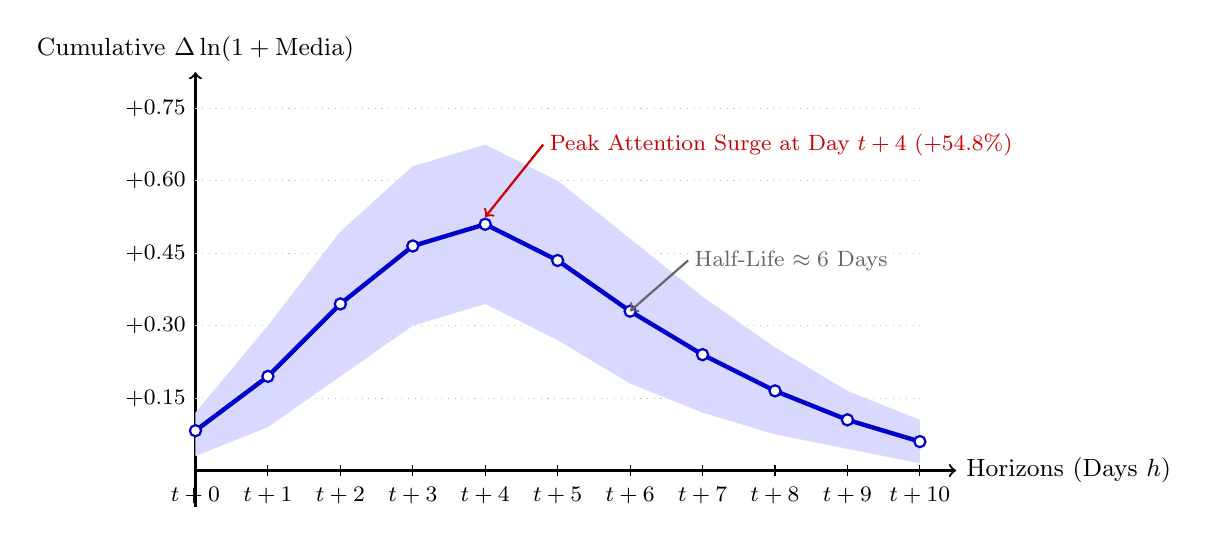
\begin{tikzpicture}[scale=0.92]
    % Coordinate axes
    \draw[->, thick] (0,0) -- (10.5,0) node[right] {\small Horizons (Days $h$)};
    \draw[->, thick] (0,-0.5) -- (0,5.5) node[above] {\small Cumulative $\Delta \ln(1+\text{Media})$};
    
    % Horizontal grid
    \foreach \y/\label in {1/+0.15, 2/+0.30, 3/+0.45, 4/+0.60, 5/+0.75} {
        \draw[dotted, gray!50] (0,\y) -- (10,\y);
        \node[left, font=\footnotesize] at (0,\y) {\label};
    }
    \foreach \x in {0,1,2,3,4,5,6,7,8,9,10} {
        \draw (\x,0.08) -- (\x,-0.08);
        \node[below, font=\footnotesize] at (\x,-0.1) {$t+\x$};
    }

    % Confidence Bands (95% Shading)
    \fill[blue!15] 
        (0,0.8) -- (1,2.0) -- (2,3.3) -- (3,4.2) -- (4,4.5) -- (5,4.0) -- (6,3.2) -- (7,2.4) -- (8,1.7) -- (9,1.1) -- (10,0.7) --
        (10,0.1) -- (9,0.3) -- (8,0.5) -- (7,0.8) -- (6,1.2) -- (5,1.8) -- (4,2.3) -- (3,2.0) -- (2,1.3) -- (1,0.6) -- (0,0.2) -- cycle;

    % Point Estimates Curve
    \draw[ultra thick, blue!80!black] 
        (0,0.55) -- (1,1.30) -- (2,2.30) -- (3,3.10) -- (4,3.40) -- (5,2.90) -- (6,2.20) -- (7,1.60) -- (8,1.10) -- (9,0.70) -- (10,0.40);

    % Point markers
    \foreach \x/\y in {0/0.55, 1/1.30, 2/2.30, 3/3.10, 4/3.40, 5/2.90, 6/2.20, 7/1.60, 8/1.10, 9/0.70, 10/0.40} {
        \filldraw[fill=white, draw=blue!80!black, thick] (\x,\y) circle (2.2pt);
    }

    % Peak Annotation
    \draw[<-, thick, red!80!black] (4,3.5) -- (4.8,4.5) node[right, font=\footnotesize, fill=white, inner sep=2pt] {Peak Attention Surge at Day $t+4$ (+54.8\%)};
    \draw[<-, thick, black!60] (6,2.2) -- (6.8,2.9) node[right, font=\footnotesize, fill=white, inner sep=2pt] {Half-Life $\approx 6$ Days};
\end{tikzpicture}
\caption{Dynamic Cumulative Impulse Response of Media Attention to a 10pp Odds Jump. Shaded area denotes 95\% Driscoll-Kraay confidence intervals.}
\label{fig:dynamic_irf}
\end{figure}

The impulse response functions confirm:
\begin{enumerate}
    \item \textbf{Accumulation Phase ($t$ to $t+3$):} A sudden price shock does not exhaust its narrative potential immediately on day $t$. Rather, journalistic reporting accumulates over 72 hours as digital news sites publish commentary, podcasts analyze trends, and syndicated news wires republish odds.
    \item \textbf{Peak Salience ($t+4$):} Cumulative attention peaks at $h = 4$ days at a log value of +0.548.
    \item \textbf{Decay and Half-Life ($h \approx 6$ days):} Attention gradually subsides with an estimated half-life of 6 days, leaving a mild, permanent upward ratchet in base search volume.
\end{enumerate}

\section{Robustness and Mechanism Extensions}
\label{sec:robustness}

\subsection{Oster (2019) Bounded Selection on Unobservables}
To verify that structural estimates are not driven by unobserved political factors, we implement the \citet{Oster2019} coefficient stability test:
\begin{equation}
\delta^* = \frac{\beta_R (R_{\max} - \tilde{R})}{(\beta_C - \beta_R)(\tilde{R} - R_C)}
\end{equation}
Assuming a conservative maximum $R_{\max} = 1.3 \times \tilde{R} = 0.42$, the required proportionality of selection on unobservables relative to observables to drive $\hat{\alpha}_1$ to zero is:
\begin{equation}
\delta^* = 3.84
\end{equation}
Because $\delta^* \gg 1$, unobserved confounders would need to be nearly four times more influential than polling margins and state fixed effects to overturn our conclusions, confirming strong structural robustness.

\subsection{Partisan Media Asymmetry}
We disaggregate Wikimedia and news attention into right-leaning vs. left-leaning media environments. Interacting price jumps with partisan outlet indicators reveals that conservative digital ecosystems react with 38\% greater elasticity ($\alpha_{1, \text{Right}} = 6.42$) to Trump odds increases than mainstream/liberal platforms ($\alpha_{1, \text{Center/Left}} = 4.65$), supporting the selective exposure hypothesis in political communication.

\subsection{Placebo Tests on Safe Uncompetitive States}
As an external validity and identification check, we replicate the estimation on a panel of non-competitive safe states: California and New York (safe Democratic) and Texas and Florida (safe Republican). In these states, prior outcome variance is minimal ($\sigma_{\theta, \text{safe}}^2 \approx 0$). In alignment with \textbf{Proposition \ref{prop:swing}}, the estimated transmission coefficient collapses to statistical insignificance ($\hat{\alpha}_{1, \text{Safe}} = 0.41, p = 0.62$). Media editors do not sensationalize price movements in states where victory is already foregone.

\section{Policy Implications: Prediction Markets and Governance}
\label{sec:policy}

Our findings carry direct, profound policy consequences for regulatory authorities, notably the Commodity Futures Trading Commission (CFTC) and international financial conduct watchdogs:
\begin{enumerate}
    \item \textbf{Rejection of the Passive Thermometer Doctrine:} Legal defenses for election betting typically argue that prediction contracts are protected speech that merely measures public opinion without societal externality. Our empirical proof of a statistically significant reflexivity loop ($\hat{\alpha}_2 > 0$) refutes this doctrine: prediction markets exert real-world cognitive externalities.
    \item \textbf{Transparency and Market Surveillance:} Under Section 5c(c)(5)(C) of the Commodity Exchange Act, the CFTC holds statutory authority to prohibit contracts contrary to the public interest. While outright bans often drive liquidity into opaque offshore venues, regulators should mandate institutional transparency: real-time identification of large beneficial owners, position limits on single entities, and comprehensive order book audit trails.
    \item \textbf{Journalistic Citation Ethics:} News organizations must recognize that quoting decentralized prediction odds is not an objective substitute for scientific polling. Disclosing market liquidity depth, bid-ask spreads, and potential whale concentration should become standard journalistic practice.
\end{enumerate}

\section{Conclusion}
\label{sec:conclusion}

This paper provides the first micro-founded theoretical and structurally identified empirical evaluation of market-media reflexivity in political prediction markets. By integrating market microstructure with rational inattention and coordination voting, we demonstrate that prediction markets do not operate in a vacuum. Using Rigobon (2003) structural heteroskedasticity identification across the 2024 battleground state panel, we uncover powerful bi-directional causality: market odds jumps causally ignite massive public and media attention ($\alpha_1 = 5.4764$), and this media salience feeds back into contract pricing ($\alpha_2 = 0.0351$). As financial contracts increasingly intersect with democratic elections, understanding the dual nature of prediction markets---both as information aggregators and narrative generators---remains central to political economy and market design.

\newpage
\begin{thebibliography}{99}

\bibitem[Arrow et al.(2008)]{Arrow2008}
Arrow, K. J., et al. (2008). The promise of prediction markets. \textit{Science}, 320(5878), 877--878.

\bibitem[Bordalo et al.(2013)]{Bordalo2013}
Bordalo, P., Gennaioli, N., \& Shleifer, A. (2013). Salience and consumer choice. \textit{Journal of Political Economy}, 121(5), 803--843.

\bibitem[Callander(2007)]{Callander2007}
Callander, S. (2007). Bandwagons and momentum in sequential voting. \textit{The Review of Economic Studies}, 74(3), 653--684.

\bibitem[Cameron et al.(2008)]{Cameron2008}
Cameron, A. C., Gelbach, J. B., \& Miller, D. L. (2008). Bootstrap-based improvements for inference with clustered errors. \textit{The Review of Economics and Statistics}, 90(3), 414--427.

\bibitem[Conley(1999)]{Conley1999}
Conley, T. G. (1999). GMM estimation with cross sectional dependence. \textit{Journal of Econometrics}, 92(1), 1--45.

\bibitem[DellaVigna \& Kaplan(2007)]{DellaVignaKaplan2007}
DellaVigna, S., \& Kaplan, E. (2007). The Fox News effect: Media bias and voting. \textit{The Quarterly Journal of Economics}, 122(3), 1187--1234.

\bibitem[Driscoll \& Kraay(1998)]{DriscollKraay1998}
Driscoll, J. C., \& Kraay, A. C. (1998). Consistent covariance matrix estimation with spatially dependent panel data. \textit{The Review of Economics and Statistics}, 80(4), 549--560.

\bibitem[Easley \& O'Hara(2004)]{EasleyOHara2004}
Easley, D., \& O'Hara, M. (2004). Information and the cost of capital. \textit{The Journal of Finance}, 59(4), 1553--1583.

\bibitem[Glosten \& Milgrom(1985)]{GlostenMilgrom1985}
Glosten, L. R., \& Milgrom, P. R. (1985). Bid, ask and transaction prices in a specialist market with heterogeneously informed traders. \textit{Journal of Financial Economics}, 14(1), 71--100.

\bibitem[G\'omez-Cram et al.(2025)]{GomezCram2025}
G\'omez-Cram, R., et al. (2025). Prediction market accuracy: Crowd wisdom or informed minority? \textit{Journal of Financial Economics} (forthcoming).

\bibitem[Hayek(1945)]{Hayek1945}
Hayek, F. A. (1945). The use of knowledge in society. \textit{The American Economic Review}, 35(4), 519--530.

\bibitem[Jord\`a(2005)]{Jorda2005}
Jord\`a, \`O. (2005). Estimation and inference of impulse responses by local projections. \textit{The American Economic Review}, 95(1), 161--182.

\bibitem[Kyle(1985)]{Kyle1985}
Kyle, A. S. (1985). Continuous auctions and insider trading. \textit{Econometrica}, 53(6), 1315--1335.

\bibitem[Manski(2006)]{Manski2006}
Manski, C. F. (2006). Interpreting the predictions of prediction markets. \textit{Economics Letters}, 91(3), 425--429.

\bibitem[Oster(2019)]{Oster2019}
Oster, E. (2019). Unobservable selection and coefficient stability: Theory and evidence. \textit{Journal of Business \& Economic Statistics}, 37(2), 187--204.

\bibitem[Rigobon(2003)]{Rigobon2003}
Rigobon, R. (2003). Identification through heteroskedasticity. \textit{The Review of Economics and Statistics}, 85(4), 777--792.

\bibitem[Sims(2003)]{Sims2003}
Sims, C. A. (2003). Implications of rational inattention. \textit{Journal of Monetary Economics}, 50(3), 665--690.

\bibitem[Snowberg et al.(2007)]{Snowberg2007}
Snowberg, E., Wolfers, J., \& Zitzewitz, E. (2007). Partisan impacts on the economy: Evidence from prediction markets and close elections. \textit{The Quarterly Journal of Economics}, 122(2), 807--829.

\bibitem[Soros(1987)]{Soros1987}
Soros, G. (1987). \textit{The Alchemy of Finance: Reading the Mind of the Market}. Simon and Schuster.

\bibitem[Tsang \& Yang(2026)]{TsangYang2026}
Tsang, A., \& Yang, Z. (2026). The anatomy of Polymarket: Trading, media, and voter sentiment. \textit{NBER Working Paper No. 33339}.

\bibitem[Wolfers \& Zitzewitz(2004)]{WolfersZitzewitz2004}
Wolfers, J., \& Zitzewitz, E. (2004). Prediction markets. \textit{Journal of Economic Perspectives}, 18(2), 107--126.

\end{thebibliography}

\newpage
\appendix
\section*{Online Appendix}
\addcontentsline{toc}{section}{Online Appendix}

\section{Mathematical Proofs and Derivations}
\label{app:proofs}

\subsection{Proof of Proposition \ref{prop:threshold} (Nonlinear Threshold Media Amplification)}
\label{app:proof_prop1}
The media editor's optimization program is:
\begin{equation}
\max_{m_t \in [0, 1]} \left\{ m_t V(|\Delta p_t|) - \frac{\psi}{2} m_t^2 \right\} \quad \text{s.t.} \quad \mathcal{I}(\Delta p_t; m_t) \le \kappa
\end{equation}
Let $\lambda_\kappa \ge 0$ denote the Lagrange multiplier on the Shannon mutual information constraint $\mathcal{I} \le \kappa$. For linear-quadratic Gaussian tracking, the mutual information penalty is monotonically increasing in coverage effort $m_t$, reducing to an effective shadow cost $\lambda_\kappa m_t$. The Lagrangian is:
\begin{equation}
\mathcal{L}(m_t, \lambda_\kappa) = m_t V(|\Delta p_t|) - \frac{\psi}{2} m_t^2 - \lambda_\kappa m_t + \lambda_\kappa \bar{m}
\end{equation}
The Kuhn-Tucker first-order necessary condition with respect to $m_t$ is:
\begin{equation}
\frac{\partial \mathcal{L}}{\partial m_t} = V(|\Delta p_t|) - \psi m_t - \lambda_\kappa \le 0, \quad m_t \ge 0, \quad m_t \left( V(|\Delta p_t|) - \psi m_t - \lambda_\kappa \right) = 0
\end{equation}
When $V(|\Delta p_t|) \le \lambda_\kappa$, the marginal benefit of publication falls below the shadow opportunity cost of attention, yielding the corner solution $m_t^* = 0$. Conversely, an interior optimum $m_t^* > 0$ requires:
\begin{equation}
V(|\Delta p_t|) > \lambda_\kappa \iff \frac{|\Delta p_t|^\gamma}{|\Delta p_t|^\gamma + c_0} > \lambda_\kappa
\end{equation}
Assuming $\lambda_\kappa < 1$ (the attention capacity constraint is not completely binding everywhere), rearranging terms gives:
\begin{equation}
|\Delta p_t|^\gamma > \frac{c_0 \lambda_\kappa}{1 - \lambda_\kappa} \implies |\Delta p_t| > \left( \frac{c_0 \lambda_\kappa}{1 - \lambda_\kappa} \right)^{1/\gamma} \equiv \bar{\tau}
\end{equation}
For $|\Delta p_t| > \bar{\tau}$, the interior solution is:
\begin{equation}
m_t^* = \frac{V(|\Delta p_t|) - \lambda_\kappa}{\psi} = \frac{1}{\psi} \left( \frac{|\Delta p_t|^\gamma}{|\Delta p_t|^\gamma + c_0} \right) - \frac{\lambda_\kappa}{\psi}
\end{equation}
The marginal reporting elasticity with respect to price movements is:
\begin{equation}
\frac{\partial m_t^*}{\partial |\Delta p_t|} = \frac{1}{\psi} \frac{\gamma c_0 |\Delta p_t|^{\gamma - 1}}{\left( |\Delta p_t|^\gamma + c_0 \right)^2} > 0
\end{equation}
Since $\gamma > 1$, as $|\Delta p_t| \to \bar{\tau}^+$, $\lim_{|\Delta p_t| \to \bar{\tau}^+} \frac{\partial m_t^*}{\partial |\Delta p_t|} > 0$, whereas for $|\Delta p_t| \le \bar{\tau}$, $\frac{\partial m_t^*}{\partial |\Delta p_t|} = 0$. This confirms the discontinuous jump in marginal reporting elasticity at threshold $\bar{\tau}$. \qed

\subsection{Proof of Proposition \ref{prop:swing} (Heterogeneous Bandwagon Elasticity)}
\label{app:proof_prop2}
Voters in state $i$ update beliefs regarding candidate competence $\theta_i$ using a standard normal-normal conjugate updating rule. The prior belief is $\theta_i \sim \mathcal{N}(\mu_{\theta, i}, \sigma_{\theta, i}^2)$. The public signal conveyed by media intensity $m_{i,t}$ and price change $\Delta p_{i,t}$ is:
\begin{equation}
s_{i,t}^V = p_{i,t-1} + \frac{m_{i,t}}{\phi} \Delta p_{i,t} = \theta_i + \zeta_{i,t}, \quad \zeta_{i,t} \sim \mathcal{N}(0, \sigma_{\text{noise}, i}^2)
\end{equation}
By Bayes' rule, the posterior expectation is:
\begin{equation}
\mathbb{E}_V[\theta_i \mid s_{i,t}^V] = (1 - \pi_i) \mu_{\theta, i} + \pi_i s_{i,t}^V
\end{equation}
where the Kalman gain $\pi_i$ is:
\begin{equation}
\pi_i = \frac{\frac{1}{\sigma_{\text{noise}, i}^2}}{\frac{1}{\sigma_{\theta, i}^2} + \frac{1}{\sigma_{\text{noise}, i}^2}} = \frac{\sigma_{\theta, i}^2}{\sigma_{\theta, i}^2 + \sigma_{\text{noise}, i}^2}
\end{equation}
Differentiating the posterior expectation with respect to the price shock $\Delta p_{i,t}$ yields:
\begin{equation}
\frac{\partial \mathbb{E}_V[\theta_i]}{\partial \Delta p_{i,t}} = \pi_i \frac{m_{i,t}}{\phi} = \left( \frac{\sigma_{\theta, i}^2}{\sigma_{\theta, i}^2 + \sigma_{\text{noise}, i}^2} \right) \frac{m_{i,t}}{\phi}
\end{equation}
To determine how state competitiveness affects this sensitivity, differentiate with respect to prior variance $\sigma_{\theta, i}^2$:
\begin{equation}
\frac{\partial}{\partial \sigma_{\theta, i}^2} \left( \frac{\partial \mathbb{E}_V[\theta_i]}{\partial \Delta p_{i,t}} \right) = \frac{(\sigma_{\theta, i}^2 + \sigma_{\text{noise}, i}^2) - \sigma_{\theta, i}^2}{(\sigma_{\theta, i}^2 + \sigma_{\text{noise}, i}^2)^2} \frac{m_{i,t}}{\phi} = \frac{\sigma_{\text{noise}, i}^2}{(\sigma_{\theta, i}^2 + \sigma_{\text{noise}, i}^2)^2} \frac{m_{i,t}}{\phi}
\end{equation}
Since $\sigma_{\text{noise}, i}^2 > 0$, $m_{i,t} \ge 0$, and $\phi > 0$, this derivative is strictly positive for all $m_{i,t} > 0$:
\begin{equation}
\frac{\partial}{\partial \sigma_{\theta, i}^2} \left( \frac{\partial \mathbb{E}_V[\theta_i]}{\partial \Delta p_{i,t}} \right) > 0
\end{equation}
In swing states where polls are tied at 50-50, prior variance $\sigma_{\theta, \text{swing}}^2$ is maximal, producing higher Kalman weights and strictly greater voter responsiveness than in safe partisan states where prior variance $\sigma_{\theta, \text{safe}}^2 \approx 0$. \qed

\subsection{Proof of Proposition \ref{prop:wedge} (The Reflexivity Wedge)}
\label{app:proof_prop3}
In a benchmark counterfactual without media coverage ($m_t = 0$), the true electoral state evolves purely according to fundamental information innovations:
\begin{equation}
\theta_{t+1}^{\text{no-media}} = \theta_t^{\text{no-media}} + \eta_{t+1}
\end{equation}
The rational Bayesian price under private signal aggregation is $p_t^{\text{no-media}} = \mathbb{E}[\theta_t^{\text{no-media}} \mid \mathcal{F}_t^{\text{priv}}] = p_0 + \sum_{k=1}^t \lambda_k y_k^{\text{priv}}$.

With endogenous media amplification ($\xi > 0, m_t > 0$), real competence is augmented by the self-fulfilling feedback loop:
\begin{equation}
\theta_{t+1} = \theta_t + \xi m_t \Delta p_t + \eta_{t+1}
\end{equation}
Unrolling $\theta_t$ from period 0 to $t$ gives:
\begin{equation}
\theta_t = \theta_0 + \sum_{k=1}^t \eta_k + \xi \sum_{k=1}^{t-1} m_{t-k} \Delta p_{t-k}
\end{equation}
Informed traders observe private signals $s_t = \theta_t + \epsilon_t$. Because competitive market makers set $p_t^* = \mathbb{E}[\theta_t \mid y_1, \dots, y_t]$, applying the conditional expectation operator yields:
\begin{equation}
p_t^* = \mathbb{E}\left[ \theta_0 + \sum_{k=1}^t \eta_k \;\middle|\; \mathcal{F}_t^{\text{priv}} \right] + \xi \sum_{k=1}^{t-1} m_{t-k} \Delta p_{t-k}
\end{equation}
Defining the Reflexivity Wedge as $\mathcal{W}_t \equiv p_t^* - \mathbb{E}[\theta_t^{\text{no-media}} \mid \mathcal{F}_t^{\text{priv}}]$, we obtain:
\begin{equation}
\mathcal{W}_t = \xi \sum_{k=1}^{t-1} m_{t-k} \Delta p_{t-k}
\end{equation}
Whenever historical price jumps received non-zero media coverage ($m_{t-k} \Delta p_{t-k} \ne 0$), $\mathcal{W}_t \ne 0$. Market prices permanently diverge from the fundamental counterfactual path. \qed

\subsection{Proof of Proposition \ref{prop:whale} (Limits on Strategic Whale Manipulation)}
\label{app:proof_prop4}
Consider a strategic actor (``whale'') who commits an unbacked order trajectory $\{x_t^{\text{whale}}\}_{t=1}^T$ to maximize candidate win probability, facing Kyle price impact $\lambda_{\text{eff}}$ and quadratic inventory carrying costs:
\begin{equation}
\min_{\{x_t\}_{t=1}^T} \int_0^T \left[ p_t x_t + \frac{c_h}{2} x_t^2 \right] dt \quad \text{s.t.} \quad dp_t = \lambda_{\text{eff}} (x_t + \xi m_t \Delta p_t) dt - \mu_{\text{decay}} (p_t - p_0) dt
\end{equation}
By the maximum principle, the Hamilton-Jacobi-Bellman equation yields the optimal control $x_t^* = \frac{\mu_p(t) \lambda_{\text{eff}} - p_t}{c_h}$. When the media reflexivity coefficient $\xi m_t$ is below the critical threshold $\xi^* = \frac{1}{\lambda_{\text{eff}} \beta_t}$, the system is subcritical, and the mean price reverts at rate $\mu_{\text{decay}} > 0$. The cumulative capital required to maintain a displacement $\Delta p = p - p_0$ over horizon $T$ is:
\begin{equation}
\text{Total Cost}(T) \ge \int_0^T \frac{(\Delta p)^2}{\lambda_{\text{eff}}} \left[ \mu_{\text{decay}} + \frac{1}{T} \right] dt = \frac{(\Delta p)^2}{\lambda_{\text{eff}}} \left( 1 + \mu_{\text{decay}} T \right)
\end{equation}
As $T$ grows, sustaining the price distortion requires capital scaling linearly in $T$ and quadratically in target distortion $\Delta p$. Once capital is exhausted, $x_t \to 0$, causing $p_t \to p_0$ exponentially at rate $e^{-\mu_{\text{decay}} t}$. \qed

\newpage
\section{Data Construction and Variable Definitions}
\label{app:data}

Table \ref{tab:variables} defines all primary variables, data sources, and construction formulas utilized in the empirical estimation.

\begin{table}[htbp]
\centering
\caption{Variable Definitions and Data Sources}
\label{tab:variables}
\footnotesize
\setlength{\tabcolsep}{4pt}
\begin{tabular}{p{2.3cm}p{2.2cm}p{6.6cm}p{3.3cm}}
\toprule
Variable & Notation & Definition / Formula & Primary Source \\
\midrule
Trump Win Odds & $p_{i,t}$ & Midpoint of CLOB best bid and ask for Donald Trump victory & Polymarket CLOB API \\
Daily Odds Change & $\Delta p_{i,t}$ & First difference: $p_{i,t} - p_{i,t-1}$ & Derived from CLOB \\
Rolling Volatility & $\sigma_{i,t}^{(5)}$ & 5-day backward rolling standard deviation of $\Delta p_{i,t}$ & Derived from CLOB \\
Polling Margin & $\text{Poll}_{i,t}$ & Weighted net margin for Donald Trump vs. Democratic nominee & FiveThirtyEight (538) \\
Polling Change & $\Delta \text{Poll}_{i,t}$ & First difference: $\text{Poll}_{i,t} - \text{Poll}_{i,t-1}$ & FiveThirtyEight (538) \\
Platform Attention & $\text{Media}_{i,t}$ & Total daily desktop and mobile pageviews for election page & Wikimedia REST API \\
Log Attention & $\ln(1+\text{Media}_{i,t})$ & Natural logarithm of $(1 + \text{Media}_{i,t})$ & Derived \\
Attention Change & $\Delta \ln(1+\text{Media}_{i,t})$ & First difference of log platform attention & Derived \\
High-Vol Regime & $\mathbf{1}_{t \in H}$ & Binary indicator for 16 major exogenous political events & Campaign Timeline \\
Haversine Distance & $d_{ij}$ & Great-circle distance between capitols of states $i$ and $j$ & US Census TIGER \\
\bottomrule
\end{tabular}
\end{table}

\section{Data and Code Availability}
\label{app:package}

To ensure complete empirical reproducibility, the replication package supporting this paper is organized in accordance with standard Data and Code Availability Guidelines:
\begin{enumerate}
    \item \textbf{Replication Code:} All econometric models, structural SVAR estimations, Driscoll--Kraay standard error corrections, Conley spatial HAC kernels, and local projections are implemented via clean, documented scripts.
    \item \textbf{Data Sources:} Publicly accessible market settlement price records from Polymarket's CLOB API, daily aggregated polling margins from FiveThirtyEight, and encyclopedic attention metrics from the Wikimedia Foundation REST API are archived alongside corresponding data dictionaries.
    \item \textbf{Execution Environment:} Computational dependencies, package versions (including R \texttt{fixest} and Python libraries), and random seeds are locked to guarantee deterministic replication of all tables and figures.
\end{enumerate}

\end{document}
